\chapter{The LHC and CMS Detector} % (fold)
\label{cha:the_lhc_and_cms_machine}

In this chapter, the working and the design parameters of the Large Hadron Collider (LHC) and one of its general purpose detector, Compact Muon Solenoid (CMS), are briefly described.


%%%%%%%%%%%%%%%%%%%%%%%%%%%%%%%%%%%%%%%%%%%%%%%%%%%%%%%%%%%%%%%%%%
\section{The Large Hadron Collider} % (fold)
\label{sec:the_large_hadron_collider}

The famous quote ``history repeats itself" applies well to the High Energy Physics (HEP) experiments. The starting point of experimental particle physics was the Rutherford $\alpha$-particle scattering, which was proposed by Ernest Rutherford and carried out by his two assistants  Hans Geiger and Ernest Marsden in early $20^{th}$ century~\cite{Hauptman2010}. In this experiment, a beam of $\alpha$-particles was fired at the thin gold foil and its scattering was observed on the photographic screen. Based on the experimental findings, they suggested the well known structure of today's atom, in which the most of the mass centred at the core of atom which is known as nucleus and the electrons  revolve around the nucleus. Hundred years after this experiment, we imploy the same techniques to explore the basic constituents matter. Just the technique changed from ``natural accelerator"\footnote{radioactivity and cosmic rays} to the ``man-made" accelerator that can accelerate particles with the speed close to the speed of light. The design and working of the particle accelerator has changed a lot over the period of time in going from MeV to GeV and then to TeV range. Nowadays, the accelerators are not only used in HEP experiments, but also extend their arenas to the medical sciences such as production of radioisotopes for cancer treatments, 3-D X-rays, etc. and to the industrial applications involving material processing, sterilization, security scan, water treatment, and many more. 

The Large Hadron Collider (LHC), as the name suggests, is  a hadron collider which can accelerate two proton beams, moving in opposite direction, to a maximum of 14 TeV energy in a 26.7 km long tunnel which is about 100 m underground spanning border areas of France and Switzerland. The LHC is the latest and the most-powerful particle accelerator and collider built to improve our understanding of fundamental physics. It started its operation on 21$^{st}$ October 2008 and is housed in the tunnel previously used by Large Electron Positron Collider (LEP). The European Organization for Nuclear Research (CERN) decided to switch this to hadron collider because of following advantages:
\begin{itemize}
    \item Hadron collider can reach a higher centre of mass energy, because of much lower synchrotron radiation \footnote{The radiation emitted by a charged particle during acceleration in a circular path is known as synchrotron radiation. As the particles lose energy in emission of this radiation an additional energy must be provided to keep the beam at constant energy.} emitted by hadrons as compared to electrons. Synchrotron radiation loss is directly proportional to $(Energy/mass)^4$.
    \item As hadrons are composite particles, they allow us to scan over wider range of energies.
\end{itemize}

Every particle accelerator has three major components:
\begin{itemize}
  \item Beam pipes
  \item Accelerating structure
  \item Magnet system
\end{itemize}
For the LHC these components are explained briefly in the following sub-sections.

%%%%%%%%%%%%%%%%%%%%%%%%%%%%%%%%%%%%%%%%%%%%%%%%%%%%%%%%%%%%%%%%%%
%%%%%%%%%%%%%%%%%%%%%%%%%%%%%%%%%%%%%%%%%%%%%%%%%%%%%%%%%%%%%%%%%%
\subsection{Beam Pipes} % (fold)
\label{sub:beam_pipes}

At the LHC, there are two beam pipes each having a diameter of $\approx$6.3 cm in which proton beams travel in opposite directions. To avoid beam instability and loss of beam particles due to collision with gas molecules; the beam pipes are kept at ultra-high vacuum\footnote{At LHC, three different vacuum systems are used. First one is used for beam pipe; second one for insulating the cryogenically cooled magnets and third one is used for insulating the helium distribution. In the latter two it just acts as a thermal insulator as the cryogenic parts are kept at 1.9 K ($\ang{-271.3}C$)} maintained at $1.013 \times 10^{-13}$ bar pressure.
% subsection beam_pipes (end)

%%%%%%%%%%%%%%%%%%%%%%%%%%%%%%%%%%%%%%%%%%%%%%%%%%%%%%%%%%%%%%%%%%
%%%%%%%%%%%%%%%%%%%%%%%%%%%%%%%%%%%%%%%%%%%%%%%%%%%%%%%%%%%%%%%%%%
\subsection{Accelerating Structure} % (fold)
\label{sub:accelerating_structure}

Another main part of any particle accelerator is its accelerating structure. An accelerator in the TeV range cannot accelerate particles from the rest to the energies of the order of TeV, in a single go.  It should go into several stages depending on the energy. At LHC, the journey of proton starts with grabbing the proton from Hydrogen gas and subsequently going into 5 different stages. The stages can be decreased but could not be decreased to just one. Here, at LHC there are five different stages before reaching to LHC and in between it serves several other experiments at each stage, which are shown pictorially in Figure~\ref{fig:OtherExpAtAccStructure}. The stages for proton acceleration are:
\begin{itemize}
    \item Grab proton source: The source of proton is Duoplasmatron~\cite{LHC-tdr-vol3}. It strips electron from hydrogen gas and creates a plasma of protons, electrons and molecular ions. This plasma expands towards the extraction electrodes and a proton beam is formed. This feeds protons to Linear accelerator-2 (LINAC2).
    \item LINAC2: It is the starting point of proton's journey in the LHC accelerator complex. Here, proton beams are accelerated to an energy of 50 $MeV$ using the radio-frequency (RF) cavities\footnote{A RF cavity is a metallic cavity that accelerates the charged particles using the electromagnetic field.}. LINAC2 further feeds to the Proton Synchrotron Booster (PSB).
    \item PSB: It takes 50 $MeV$ proton beams from LINAC2 and accelerates them to 1.4 $GeV$ for injection into Proton Synchrotron (PS).
    \item PS: It is one of the key component in the LHC accelerator complex. It increases the energy of protons up-to 25 $GeV$ and feed them to super proton synchrotron (SPS).
    \item SPS: It has a circumference of 7 $km$ where protons are accelerated to an energy of 450 $GeV$. Then via two transmission lines protons are further injected into LHC ring.
    \item LHC: It accepts the two proton beams from SPS which are injected into opposite directions in two parallel pipes. In LHC, proton beams can be accelerated up-to 7 $TeV$.
\end{itemize}
The CERN accelerator complex is shown in Figure~\ref{fig:CERN-accelerator-complex}.  

% subsection accelerating_structure (end)
\begin{figure}[!htbp]
	\centering
	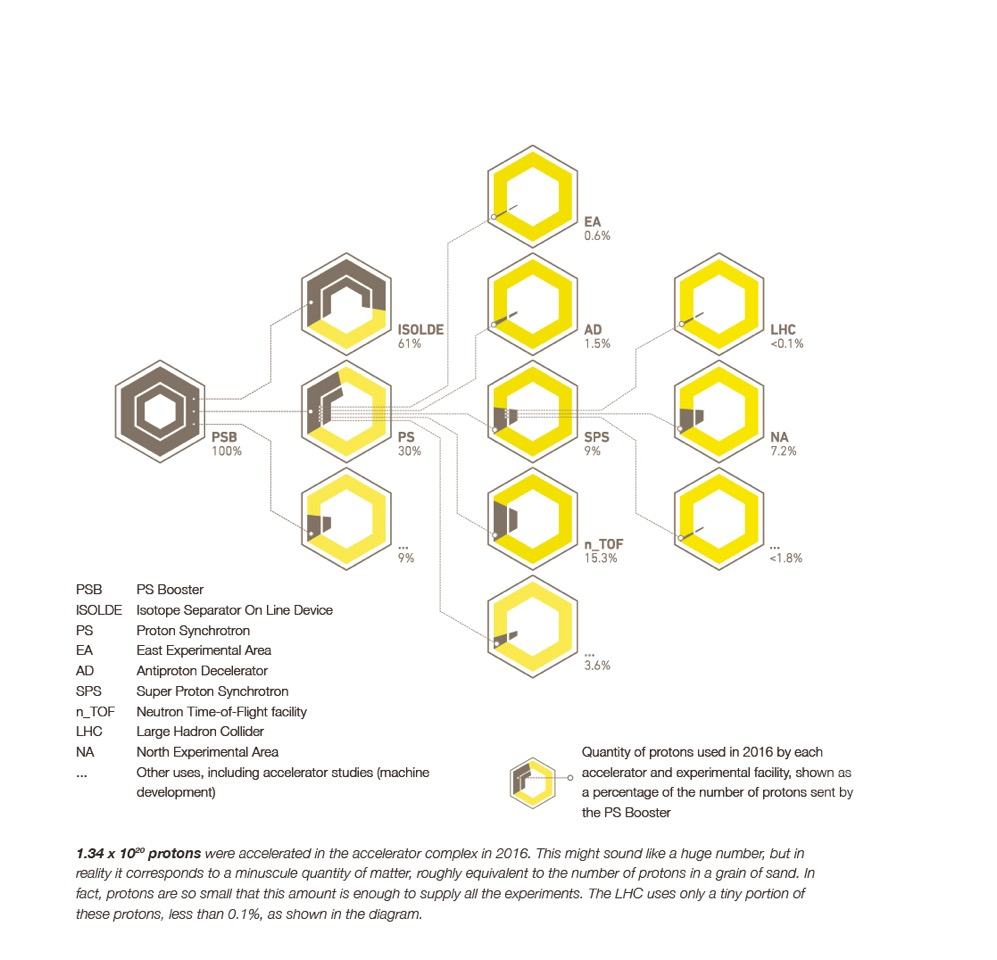
\includegraphics[width=1.0\textwidth]{figures/LHC/distribution_of_protons_en.jpg}
	\caption{Other experiments at the LHC accelerating chain \cite{OtherExpAtLHCAcceleratingChain}}
	\label{fig:OtherExpAtAccStructure}
\end{figure}
\begin{figure}[!htbp]
	\centering
	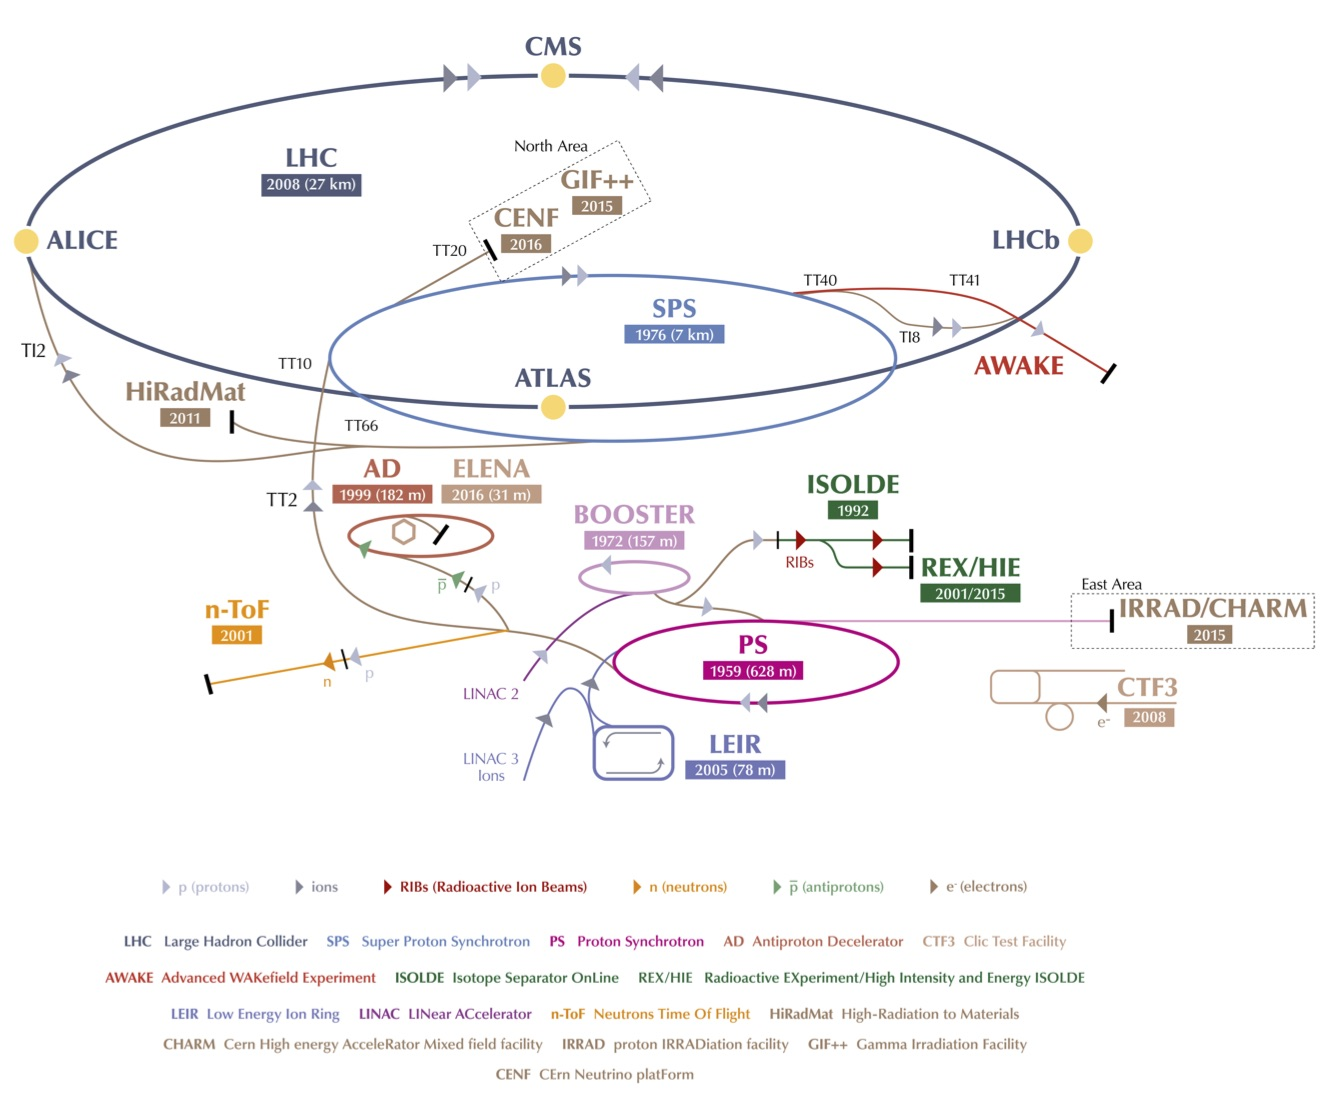
\includegraphics[width=1.15\textwidth,height=19cm]{figures/LHC/CERN_Accelerator_Complex-v2016.jpg}
	\caption{LHC accelerator chain along with all its other experiments which uses proton beam from other parts of accelerator either from PSB, PS or SPS\cite{Fig-CERN-accelerator-complex}}
	\label{fig:CERN-accelerator-complex}
\end{figure}
%%%%%%%%%%%%%%%%%%%%%%%%%%%%%%%%%%%%%%%%%%%%%%%%%%%%%%%%%%%%%%%%%%
%%%%%%%%%%%%%%%%%%%%%%%%%%%%%%%%%%%%%%%%%%%%%%%%%%%%%%%%%%%%%%%%%%
\subsection{Magnet System}
As the LHC is a circular collider; magnet system is one of the core parts and gives particles a circular trajectory in the LHC beam pipes. To be economical LHC has been made in eight arcs and eight straight sections instead of a perfect circle. Apart from bending the beam, it is also necessary to focus the two proton beams this is accomplished using a pair of quadrupole magnets, where the first magnet focus the magnet while other focuses the beam height as shown in Figure~\ref{fig:QuadrupoleMagnet}. A total of 858 quadrupole magnets are installed in LHC to keep the beams focused. Sextuple magnets are also used for proper focusing as every proton in the beam is not exactly with the same energy and on the same path. Several other magnetic multi-poles are used to keep the beam focused  in case the beam suffers from gravitational interactions over protons, electromagnetic interactions among bunches, electron clouds from pipe wall, and so on. Different types of magnets used in LHC are listed here \cite{WebLink:LHC_magnets}. Besides, there are eight sets of ``inner triplets" used at the four interaction points (IPs) to focus the beams during the collisions, to increase the luminosity. The size of bunch goes from 0.2 mm to 17 $\mu m$ at the interaction point of ATLAS or CMS. At the interaction point of ALICE or LHCb it is 71 $\mu m$. Summary of important parameters of LHC is given in Table~\ref{table:LHC-parameters}.
\begin{figure}[!htbp]
	\centering
	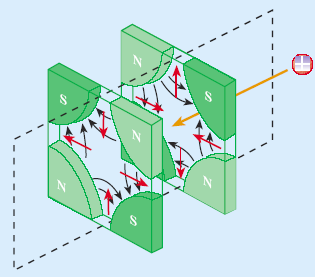
\includegraphics[width=0.65\textwidth]{figures/LHC/quadrupole_magnet_pair.png}
	\caption{Pair of quadrupole magnets.}
	\label{fig:QuadrupoleMagnet}
\end{figure}
% \begin{figure}[!htbp]
% 	\centering
% 	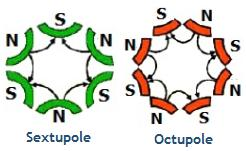
\includegraphics[width=0.95\textwidth]{figures/LHC/sextupole-octupole.jpg}
% 	\caption{Sextupole and octupole}
% 	\label{fig:sextupole-octupole}
% \end{figure}



\begin{table}
\vspace{-5.2em}
\centering
\begin{tabular}[!htbp]{l c}
\hline
{\bf Parameters} & {\bf Value} \\
\hline
Circumference of LHC ring   &   26658.883 m \\
\hline
Maximum dipole magnetic field   & 8.33 T \\
Dipole operating temperature    & 1.9 K \\
\hline
Maximum stored energy per beam (nominal) &   362 MJ \\
Maximum stored energy per beam  (2012) &   143 MJ \\
Maximum stored energy per beam  (2016) &   266 MJ \\
\hline
Beam energy at Injection    & 450 GeV \\
Beam energy at collision (nominal) &    7 TeV \\
Beam energy at collision (2012)     &   4 TeV \\
Beam energy at collision (2016)     &   6.5 TeV \\
\hline
Maximum instantaneous luminosity (nominal)  &   $10^{34}$ cm$^-2$ s$^{-1}$ \\
Maximum instantaneous luminosity (2012)     &   $7.7 \times 10^{33}$ cm$^-2$ s$^{-1}$ \\
Maximum instantaneous luminosity (2016)     &   $1.4 \times 10^{34}$ cm$^-2$ s$^{-1}$ \\
\hline
Number of bunches per proton beam (nominal) &   2808 \\
Number of bunches per proton beam (2012)    &   1380 \\
Number of bunches per proton beam (2016)    &   2076 \\
Maximum number of protons per bunch         &   $1.6 \times 10^{11}$ \\
\hline
Protons/bunch (average at start of collision) (nominal)   &   $1.15 \times 10^{11}$ \\
Protons/bunch (average at start of collision) (2012)  &   $1.5 \times 10^{11}$ \\
Protons/bunch (average at start of collision) (2016)  &   $1.1 \times 10^{11}$ \\
\hline
Bunch collision frequency (nominal)         &   40 MHz  \\
Bunch collision frequency (2012)            &   20 MHz  \\
Bunch collision frequency (2016)            &   40 MHz  \\
\hline
Bunch length (at injection)   &   1.7 ns \\
Bunch length (at collision)   &   1.05 ns \\
Energy spread (at injection)   &   1.9$\times 10^{-3}$ \\
Energy spread (at collision)   &   0.45$\times 10^{-3}$  \\
\hline
Half crossing angle  (nominal)   & 143 $\mu rad$ \\
Half crossing angle  (2012)   & 146 $\mu rad$ \\
Half crossing angle  (2016)   & 185 $\mu rad$ \\
\hline
$\beta *$  (nominal) &   0.55 m\\
$\beta *$   (2012)&   0.6 m\\
$\beta *$   (2016)&   0.4 m\\
\hline
RMS beam size at IP1 \& IP5 &   17 $\mu m$ \\
RMS beam size at IP2 \& IP8 &   71 $\mu m$ \\
\hline
$\epsilon_n$(transverse emittance, RMS, normalized) (at injection) &   3.5 $\mu$m\\
$\epsilon_n$(transverse emittance, RMS, normalized) (at collision point) &   3.75 $\mu$m\\
\hline
total longitudinal emittance (at injection) & 1.0 eVs \\
total longitudinal emittance (at collision) & 2.5 eVs \\
\hline
Average mean pile-up (nominal) &   25 \\
Average mean pile-up (2012) &    21 \\
Average mean pile-up (2016) &    27 \\
\hline
Energy loss per turn at 14 TeV              &   7 keV   \\
Energy loss per turn for electrons at 104.6 GeV          &  40,000 keV     \\
% synchtron radiation for electrons: Reference: Particle Physics Experiments at high energy colliders by John Hauptman
\end{tabular}
\caption{LHC technical parameters for proton-proton collisions: nominal, 2012 and 2016 values.\cite{Bruce2016, Schoerner-Sadenius2015, LHC-parameters-2016, LHC-tdr-vol1, cms-lumi-public-results}.}
\label{table:LHC-parameters}
\end{table}

%%%%%%%%%%%%%%%%%%%%%%%%%%%%%%%%%%%%%%%%%%%%%%%%%%%%%%%%%%%%%%%%%%
%%%%%%%%%%%%%%%%%%%%%%%%%%%%%%%%%%%%%%%%%%%%%%%%%%%%%%%%%%%%%%%%%%
\subsection{Key requirements of a particle accelerator} % (fold)
\label{sub:few_key_requirements}

The HEP collider is characterised based on two parameters centre of mass energy and the luminosity. The production rate of heavier particles like Higgs increases with the centre of mass energy. The luminosity is proportional to the number of events per second so it should be maximised. Luminosity is defined as:
\begin{equation}
    L = \frac{k_bN_b^2f_{rev}\gamma}{4 \pi \epsilon_n \beta^*}
\end{equation}
Where,\\
\hspace{2 cm}$k_b$ is the number of bunches per ring,\\
\hspace{2 cm}$N_b$ is the number of protons per bunch,\\
\hspace{2 cm}$f_{rev}$ the revolution frequency,\\
\hspace{2 cm}$\epsilon_n$ is the normalised RMS transverse beam emittance (same in both )\\
\hspace{2 cm}$\beta^*$ is the beta-function at the interaction point\\

Based on the definition of luminosity, we can maximise it by following ways:
\begin{itemize}
    \item By decreasing beam emittance, $\epsilon_n$.
    \item By improving the cryogenic system: As the factor $k_b.N_b$ is limited by thermal energy produced by synchrotron radiation.
    \item By decreasing beam-beam effect~\cite{Herr2014,Papotti2014}. As it scales with $N_b/ \epsilon_n$ which causes the spread in betatron tunes~\cite{Dubouchet2013}.
    \item Also, the space charge~\cite{Oeftiger2016} scales with $N_b/ \epsilon_n$.
\end{itemize}
% subsection few_key_requirements (end)

% section the_large_hadron_collider (end)

%%%%%%%%%%%%%%%%%%%%%%%%%%%%%%%%%%%%%%%%%%%%%%%%%%%%%%%%%%%%%%%%%%
\section{Experiments at the LHC} % (fold)
\label{sec:experiments_at_the_lhc}

At the LHC there are four IPs where the two proton beams are made to collide. At every IP one detector is placed. They are ATLAS, CMS, ALICE, and LHCb as shown in Figure~\ref{fig:LHCgeometry}. Also, there are two more small detectors LHCf and TOTEM installed close to the IP of the two main detectors ATLAS and CMS respectively.
\begin{figure}[!htbp]
	\centering
	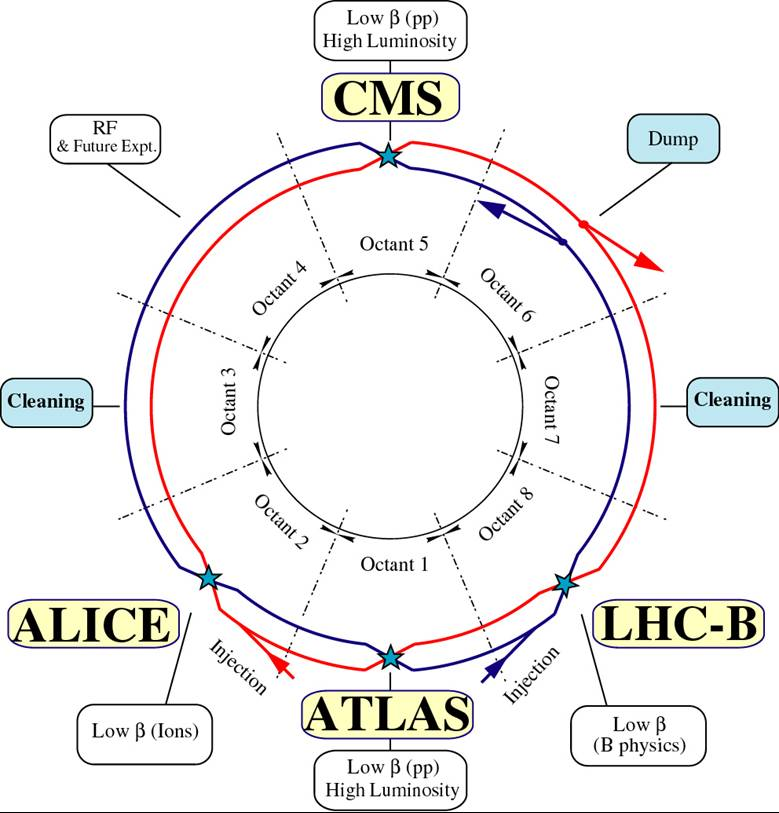
\includegraphics[width=0.81\textwidth]{figures/LHC/lhc-schematic.jpg}
	\caption{LHC geometry with arcs and straight sections.}
	\label{fig:LHCgeometry}
\end{figure}
\newline
{\bf ATLAS} (A Toroidal LHC Apparatus) and {\bf CMS} (Compact Muon Solenoid) are the two large general-purpose\footnote{Here, general purpose means this machines will be used for many different kind of physics searches.} detectors having similar design and goal. CMS detector have been described in detail in Section~\ref{sec:cms_experiment}. The main difference in the two is in their magnet systems. This is motivated by the momentum resolution of muons. The momentum resolution for muons, $\Delta p_T/p_T$, is proportional to  $B^{-1}L^{-2}$, where B is magnetic field and L is the lever arm defined as the distance of momentum measurement from the IP of detector. So, to improve the momentum resolution there are two possible choices.

\begin{enumerate}
	\item Increase the magnetic field with compact design, or
	\item Work with low magnetic field with long lever arm
\end{enumerate}

There is also a third possibility to improve the momentum resolution by increasing the leaver arm as well as magnetic field, but it increases the cost of the detector by several factors. So, CMS chooses the first point, i.e., to increase the magnetic field with compact design\footnote{This is why there is word {\bf compact} in the name of CMS.} while ATLAS chooses the design with low magnetic field with long lever arm.

% ATLAS has an eight toroidal magnets combined with a smaller inner solenoid while CMS has a powerful solenoid magnet only.

{\bf ALICE} (A Large Ion Collider Experiment) is a heavy-ion detector. It is specially designed for the study of strongly interacting matter at high densities in quark-gluon plasma phase.

{\bf LHCb} (Large Hadron Collider beauty) is made asymmetrically with respect to the IP of the detector. It is designed specially to investigate the matter-antimatter asymmetry through the study of b-quarks.

{\bf LHCf} (Large Hadron Collider forward) and {\bf TOTEM} (TOTal cross-section, Elastic scattering and diffraction dissociation Measurement at the LHC) are there for the study of forward physics\todo[fancyline]{define forward physics}.
% section experiments_at_the_lhc (end)

% %%%%%%%%%%%%%%%%%%%%%%%%%%%%%%%%%%%%%%%%%%%%%%%%%%%%%%%%%%%%%%%%%%
\section{CMS Detector} % (fold)
\label{sec:cms_experiment}
The design and components of a HEP detector depends upon the physics goals and operation parameters of the particle accelerator. In case of the CMS detector, following challenges are imposed from the LHC:
\begin{itemize}
	\item \textbf{High luminosity:} A high value of  delivered luminosity that implies every-time the two proton bunches cross each other there will be more than one p-p interactions\footnote{More than one p-p interaction in one bunch crossing is known as pile-up. It can be theoretically estimated as the product of inelastic p-p cross-section ($\sigma_{inel}$), instantaneous luminosity ($L$) and the mean time interval between two collision, ($< t >$). \begin{equation}
		mean~pile-up = \sigma_{inel} \times L \times <t>
	\end{equation}}. Given this, there will be more than $\mathcal{O}(1000)$ particles passing through detector during every p-p collision. Thus, the detector should be highly granular which results in increased number of readout channels that should be synchronised with LHC clock.
	\item \textbf{Response time:} At LHC, the two proton beams cross each other every 25 ns. So, the response time of all the sub-detector systems should be less than 25 ns.
	\item \textbf{Radiation hardness:} At every 25 ns the detectors are bombarded with more than 1000 particles so all the sub-detectors should be radiation hard including its electronics, cables, glue, screws, and so on.
\end{itemize}

Restrictions imposed on detector from the physics goals of the LHC:

\begin{itemize}
	\item Good muon identification and momentum resolution ($\approx$ 1\% at 100 GeV).
	\item Efficient triggering and tracking of b-jets and $\tau$'s.
	\item Highly efficient and granular electromagnetic calorimeter to detect and measure energies of electrons and photons.
	\item Good missing transverse energy resolution and di-jet mass resolution requires a ``hermetic'' hadron calorimeter with full geometric coverage and fine lateral segmentation.
\end{itemize}

% When the two beam of proton collides then thousands of particles are produced and out of them only 9 particles are of interest from detector construction point of view. They are photons ($\gamma$), electrons ($e$), muons ($\mu$), pions ($\pi^{\pm}$), kaon ($K^{\pm},~K_L,~K_S$), protons ($p$), and neutrons ($n$). Out of rest there are three neutrinos which interacts only weakly that do not interact in light mass HEP detectors and others are short lived particles. So, 

Based on the above conditions CMS detector is designed in a cylindrical shape having each detector on top of the other with beam pipe at the centre. To have a full geometric coverage, it is designed with a barrel region and two endcap regions. Main part of the CMS detector is its superconducting magnet system, capable of producing a highly uniform magnetic field of 4T to accurately measure the high momentum particles, while the muon detector system are kept outside the magnet but sandwiched in its return yoke. While the tracking system and calorimeters are placed inside the magnet. CMS detector design is shown in Figure~\ref{fig:CMS-detector}.
\begin{figure}[!htbp]
	\centering
	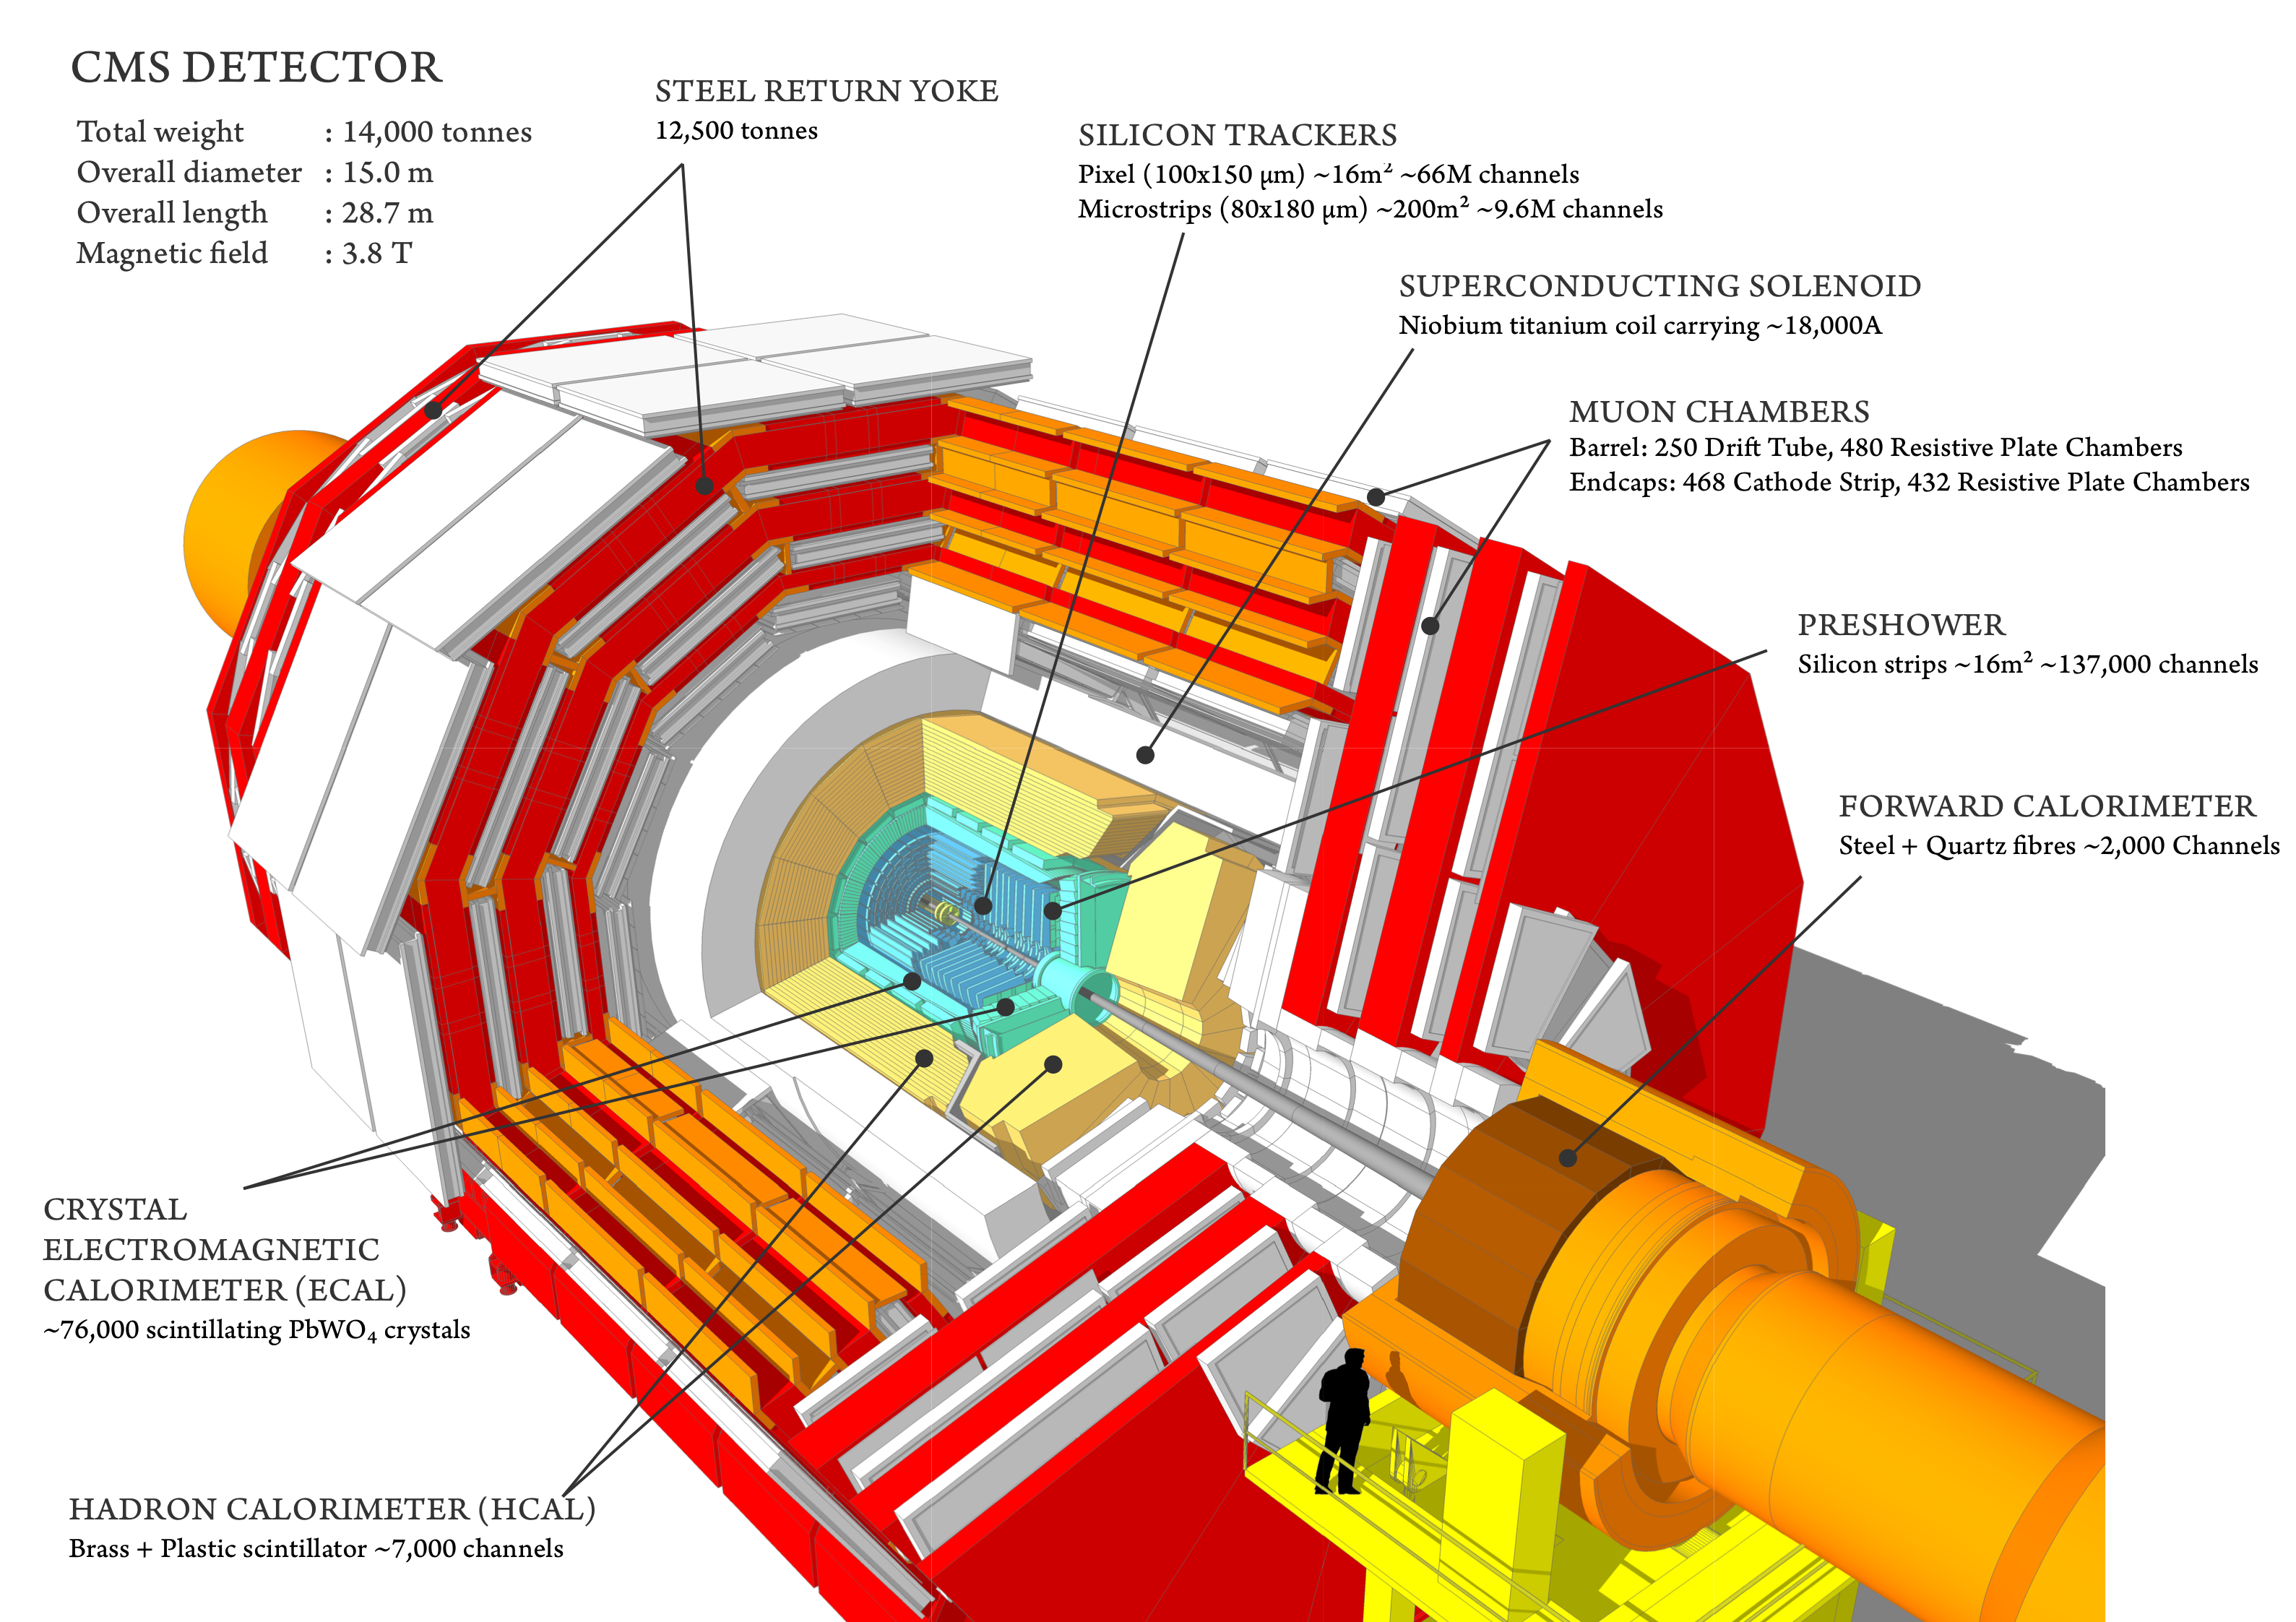
\includegraphics[width=0.95\textwidth]{figures/LHC/cms_120918_03.png}
	\caption{CMS detector drawing}
	\label{fig:CMS-detector}
\end{figure}

\subsection{Coordinate System} % (fold)
\label{sub:coordinate_system}
Right handed coordinate system is used at the CMS detector, having origin at the nominal IP (Figure~\ref{fig:cms-coordinate-system}). Z-axis is considered along the beam direction in such a way so that x-axis will point radially to the centre of LHC ring and y-direction is pointing upwards. The azimuthal angle, $\phi$, is measured in the x-y plane from x-axis and the polar angle, $\theta$, is measured from the z-axis. Instead of describing a particle at some polar angle we prefer to use the variable pseudo-rapidity. It is defined as 
\begin{equation}
	\eta = -ln\bigg[tan\Big(\frac{\theta}{2}\Big)\bigg]
\end{equation}
In the hadron collider use of pseudo-rapidity was motivated from the invariance of its difference, $\Delta \eta$, with respect to the particle boost direction. Also, the particle density remains constant in barrel region of the detector, measured in equal rapidity intervals.

\begin{figure}[htbp]
	\centering
	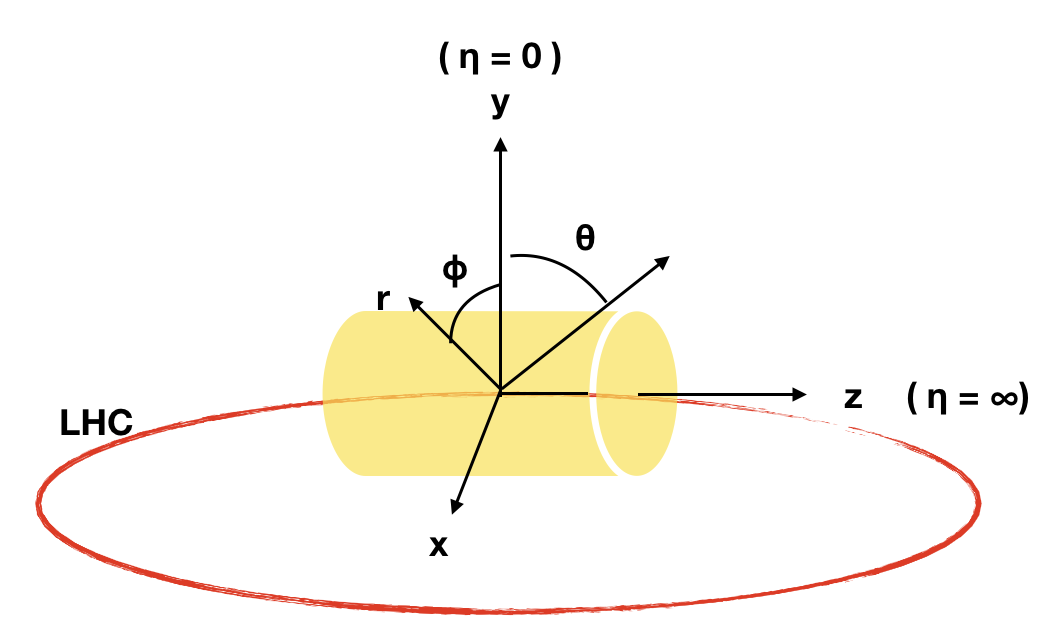
\includegraphics[width=0.95\textwidth]{figures/LHC/CMS-coordinate-system.png}
	\caption{Right handed coordinate system used by CMS.}
	\label{fig:cms-coordinate-system}
\end{figure}

% subsection coordinate_system (end)
%%%%%%%%%%%%%%%%%%%%%%%%%%%%%%%%%%%%%%%%%%%%%%%%%%%%%%%%%%%%%%%%%%
%%%%%%%%%%%%%%%%%%%%%%%%%%%%%%%%%%%%%%%%%%%%%%%%%%%%%%%%%%%%%%%%%%
\subsection{CMS sub-systems} % (fold)
\label{sub:cms_sub_systems}

%%%%%%%%%%%%%%%%%%%%%%%%%%%%%%%%%%%%%%%%%%%%%%%%%%%%%%%%%%%%%%%%%%
%%%%%%%%%%%%%%%%%%%%%%%%%%%%%%%%%%%%%%%%%%%%%%%%%%%%%%%%%%%%%%%%%%
\subsubsection{Magnet} % (fold)
\label{ssub:magnet}
Magnet system of CMS consists of a superconducting solenoid magnet which is 12.5 m in length and has an inner diameter of 6m. The size of solenoid is large as the tracker, electromagnetic calorimeter and hadron calorimeter are placed inside the solenoid. In barrel region it generates homogeneous magnetic field of 3.8 T. The high magnetic field ensures the appropriate bending power for the highly energetic charged particles to precisely measure their momentum. Outside the solenoid iron yoke is placed for the returning magnetic field. The magnetic field strenght inside the iron yoke is 2 T. Figure~\ref{fig:CMS-magnet} shows the CMS magnet.

\begin{figure}[!htbp]
	\centering
	\includegraphics[width=0.95\textwidth]{figures/LHC/CMS_magnet.jpg}
	\caption{CMS Magnet system}
	\label{fig:CMS-magnet}
\end{figure}

% subsubsection magnet (end)
%%%%%%%%%%%%%%%%%%%%%%%%%%%%%%%%%%%%%%%%%%%%%%%%%%%%%%%%%%%%%%%%%%
%%%%%%%%%%%%%%%%%%%%%%%%%%%%%%%%%%%%%%%%%%%%%%%%%%%%%%%%%%%%%%%%%%
\subsubsection{Tracker} % (fold)
\label{ssub:tracker}
Tracker is the first detector that encounters the particles emerging from the p-p collisions. Its purpose is to measure precisely the tracks of all charged particles crossing it. Also, it helps to reconstruct the secondary vertices to tag heavy flavour particles like b-jets or tau leptons. The particle rate is highest in the tracker. So, it should be highly granular and response time should be fast. This condition results in high density of on-detector electronics and this implies a large amount of materials that conflicts with the aim of low material to reduce the multiple scattering, bremsstrahlung, photon conversion and nuclear interactions. Thus, the type, design and number of layers of tracker is the trade-off between the performance, the amount of material, and the cost. Considering these things in mind CMS collaboration decided to have first three layers of silicon pixel detector to precisely measure the primary vertex, secondary vertex and the impact parameter with a total surface area of 1 $m^2$ and 66 million pixels followed by 10 layers of  silicon micro-strip detector covering a total area of 200 $m^2$. Tracker has length of 5.8 m and outer diameter 2.6 m and acceptance is up to $|\eta|<2.5$. Tracker's cross sectional view is shown in Figure~\ref{fig:tracker-cross-section}.

\begin{figure}[!htbp]
	\centering
	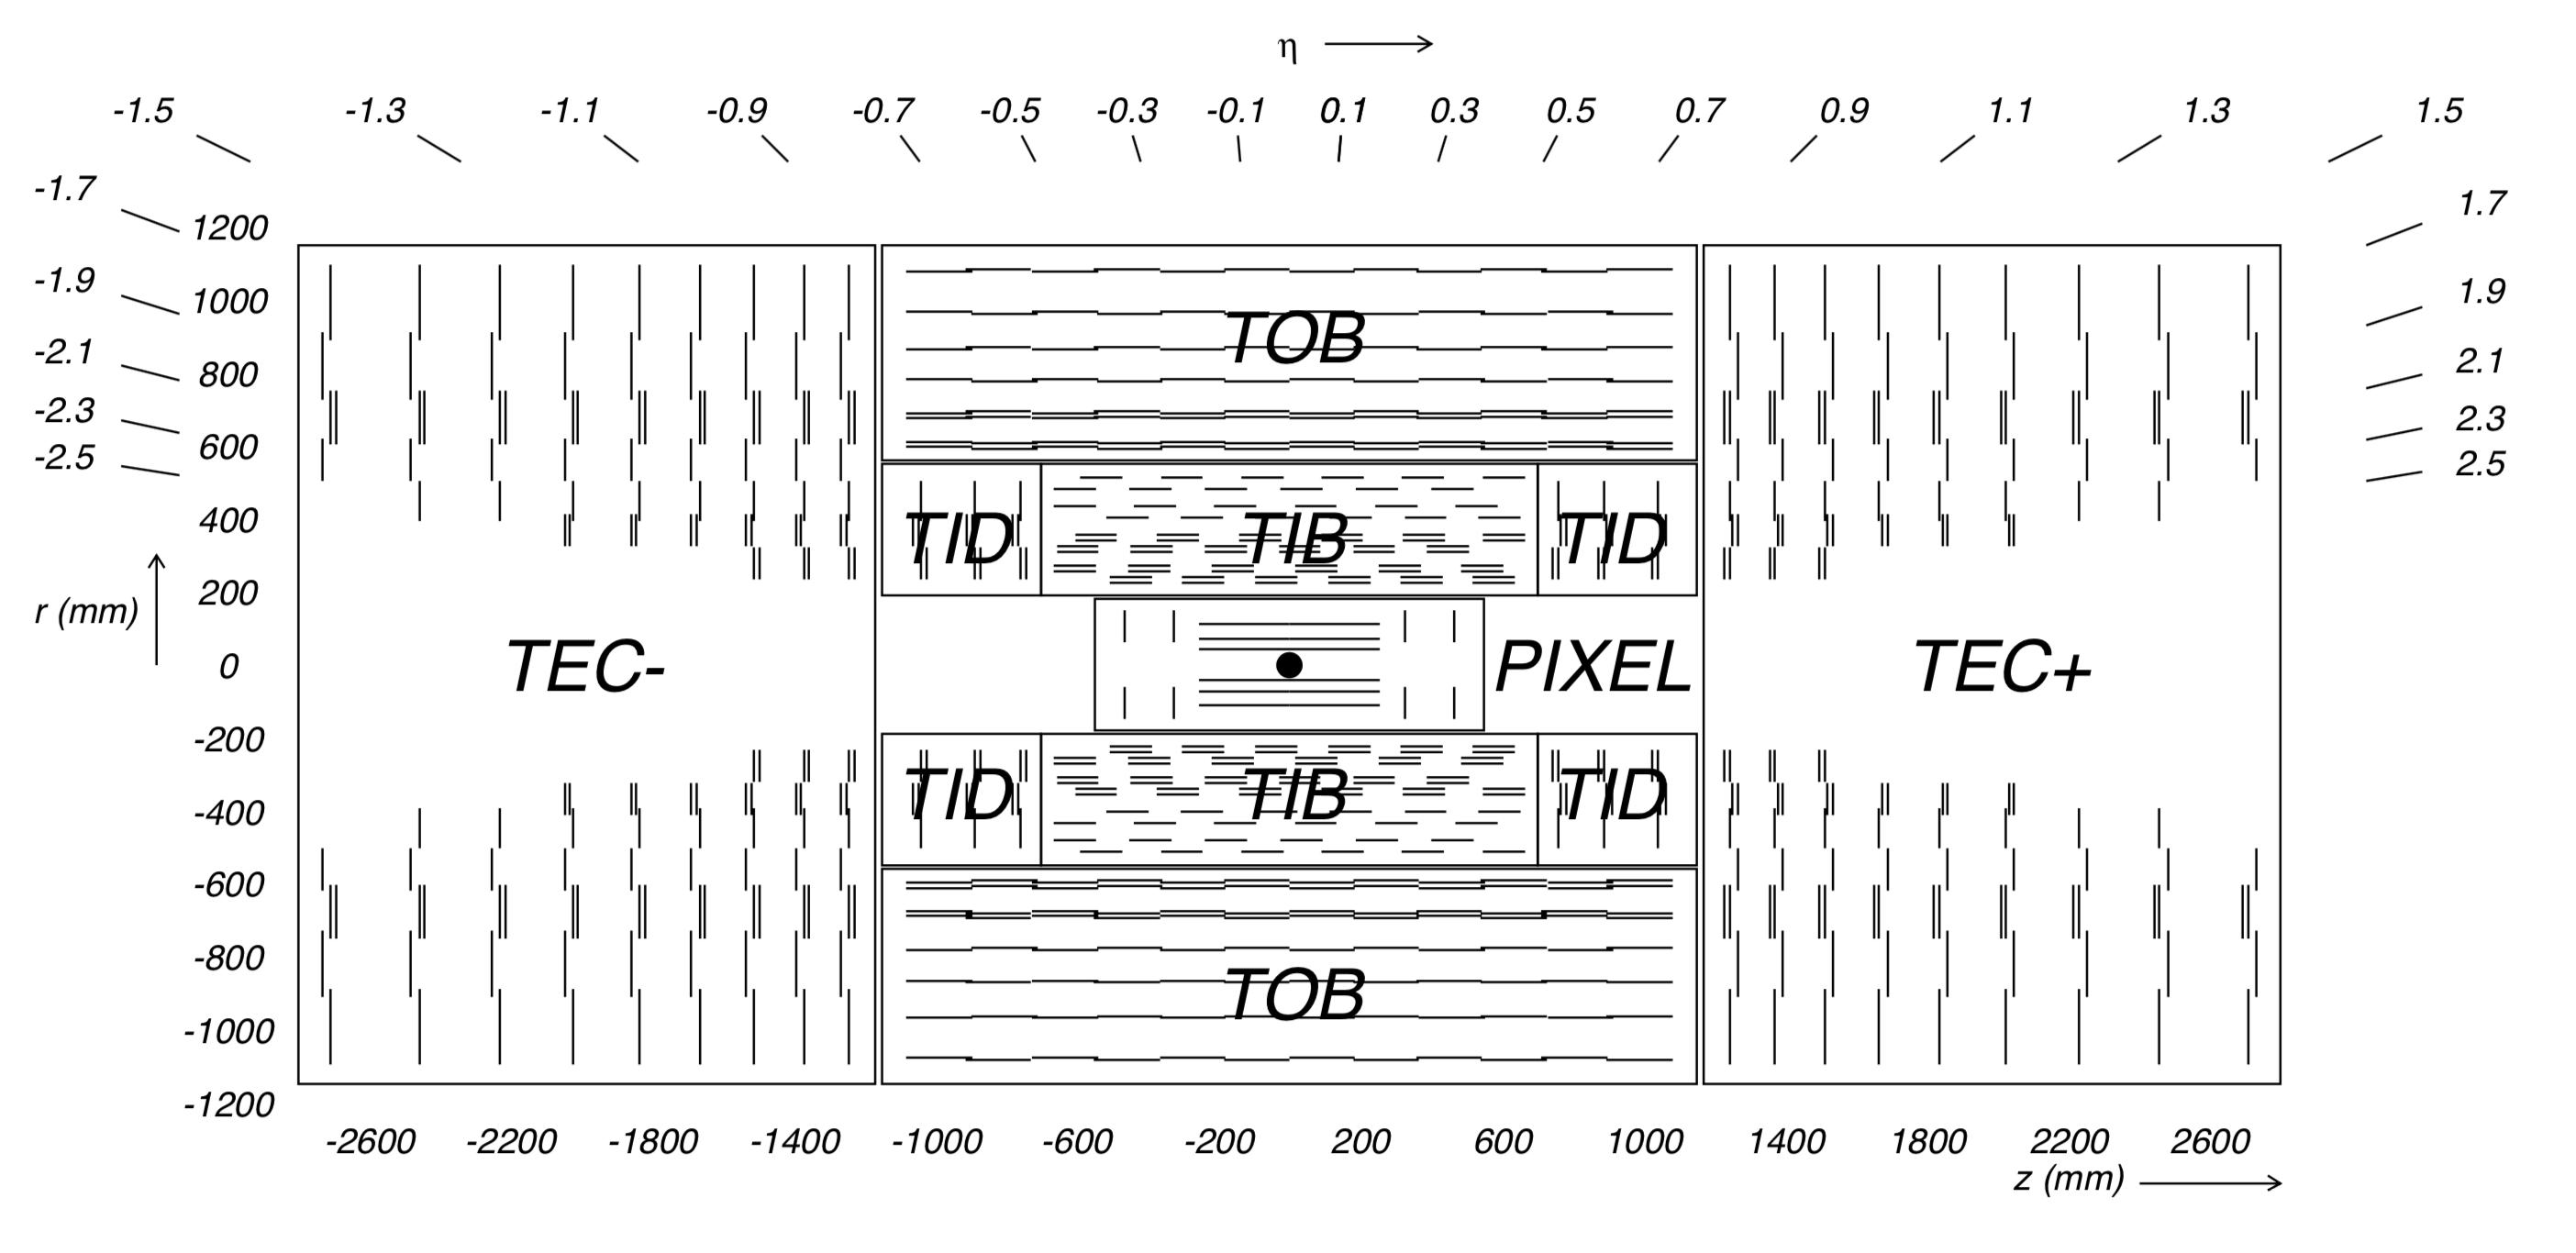
\includegraphics[width=0.95\textwidth]{figures/LHC/tracker-cross-section.png}
	\caption{Systematic cross section view of CMS tracker showing silicon pixel and strip detectors. Double line shows back-to-back modules that delivers stereo hits.}
	\label{fig:tracker-cross-section}
\end{figure}
% subsection tracker (end)

%%%%%%%%%%%%%%%%%%%%%%%%%%%%%%%%%%%%%%%%%%%%%%%%%%%%%%%%%%%%%%%%%%
%%%%%%%%%%%%%%%%%%%%%%%%%%%%%%%%%%%%%%%%%%%%%%%%%%%%%%%%%%%%%%%%%%

\subsubsection{Calorimetry} % (fold)
\label{ssub:calorimetry}
In general, the calorimeter is a device that measures the energy of particles by absorbing. The CMS detector uses two different type of calorimeter based on their interaction. They are Electromagnetic CALorimeter (ECAL) and Hadronic CALorimeter (HCAL). ECAL as the name suggest it is designed to measures the particles (electrons and photons) that primly interact via electromagnetic interaction while HCAL is designed to measure particles that interact via strong nuclear interactions.\\\\
ECAL is placed after tracker for the detection of  electrons and photons. It is a homogeneous calorimeter made from lead tungstate ($PbWO_4$) crystals, having a coverage up-to $\eta < 3.0$ including pre-shower system in forward region. The scintillation produced in barrel region is detected by Avalanche photo-diodes and in endcaps it is collected by vacuum photo-triodes. In terms of radiation length\footnote{Radiation length is defined as the mean length travelled by particle to reduce its energy by the factor of 1/e.}, $X_0$, its thickness is 25$X_0$ which guarantees almost full shower containment.\\\\
In between ECAL and magnet system, brass/scintillator sampling HCAL with coverage up to $\eta < 3.0$ is placed. To have a full geometric coverage HCAL is extended up to $\eta < 5.0$ using forward sampling iron/quartz-fibre calorimeter. This is crucial to measure the (missing) transverse energy of the event.

% The energy resolution of the ECAL can be parameterized  
% subsubsection calorimetry (end)


%%%%%%%%%%%%%%%%%%%%%%%%%%%%%%%%%%%%%%%%%%%%%%%%%%%%%%%%%%%%%%%%%%
%%%%%%%%%%%%%%%%%%%%%%%%%%%%%%%%%%%%%%%%%%%%%%%%%%%%%%%%%%%%%%%%%%
\subsubsection{The Muon System} % (fold)
\label{sub:the_muon_system}
From the name of CMS detector it is evident that the precise detection of muons is one of its main target. It is motivated by the presence of muons in the final state of many interesting physics processes, such as, the decay of Higgs boson into ZZ which subsequently decay in four leptons and especially, the case where all 4 leptons are muons is refereed to as the ``gold plated'' channel as we can detect muons efficiently over higher background contributions at LHC. At CMS, muon system serves three different functions viz. identification, momentum measurement and triggering of muons. The strong superconducting magnet system with its return yoke of CMS, helps to acquire good momentum measurement and triggering capabilities. The return yoke of magnet system also serves as the hadron absorber. Only muons leave their tracks in the muon detector system, as all other particles are already absorbed by the calorimeters. Thus, the appearance of charged particle in the muon system signifies that it can only be muons. The track left by muon in the CMS detector is illustrated in Figure~\ref{fig:muon-system-cross}. 
\begin{figure}[!htbp]
	\centering
	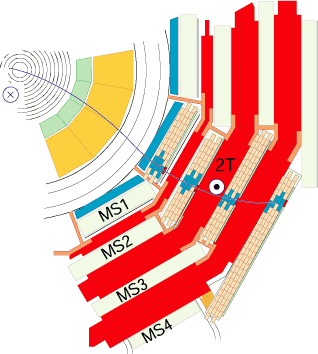
\includegraphics[width=0.55\textwidth]{figures/LHC/MuStations.png}
	\caption{A muon leaves curved trajectory in LHC and the bending changes as the magnetic field direction of solenoid inside and outside are opposite.}
	\label{fig:muon-system-cross}
\end{figure}
The layout of the CMS muon detector system is shown in Figure~\ref{fig:muon-system-layout}. Three different types of gaseous detectors used for the muon system which were chosen based on the background level, muon rate, uniformity and magnitude of magnetic field. Drift tubes are used as tracking detector in the barrel region with relatively lower magnetic field intensity and which have lower background rates as compared to the endcaps. 
For the endcap regions Cathode Strip Chamber (CSC) are employed as they are provide precise information about muons momentum and time information even in high radiation environment. The pseudo-rapidity coverage of DTs is $|\eta|<1.2$ and for CSCs is $0.9<|\eta|<2.4$. Along with DTs and CSCs, Resistive Plate Chamber (RPC) detectors are also installed to have a fast dedicated  muon triggering system in both barrel and endcap region up to $|\eta|<1.6$~\cite{muon-tdr}. The CMS muon detector system covers the geometric region up-to $|\eta|<2.4$ but RPCs are deployed up-to $|\eta|<1.6$ as RPCs cannot withstand the radiation level after pseudo-rapidity region of 1.6. Thus to reconstruct muons in pseudo-rapidity region higher than 1.6, CMS collaboration decided to employ Gas Electron Multiplier (GEM) detectors in region  $1.6<|\eta|<2.2$, which is able to provide good space resolution and time resolution even in high environment radiation during Long Shutdown-2 (LS2, 2019-2020). The pseudo-rapidity range is limited to $|\eta|<2.2$ because of space constrains. GEM  detectors are described in details in Chapter~\ref{ch:gem}.
\begin{figure}[!htbp]
	\vspace{-3.2em}
	\centering
	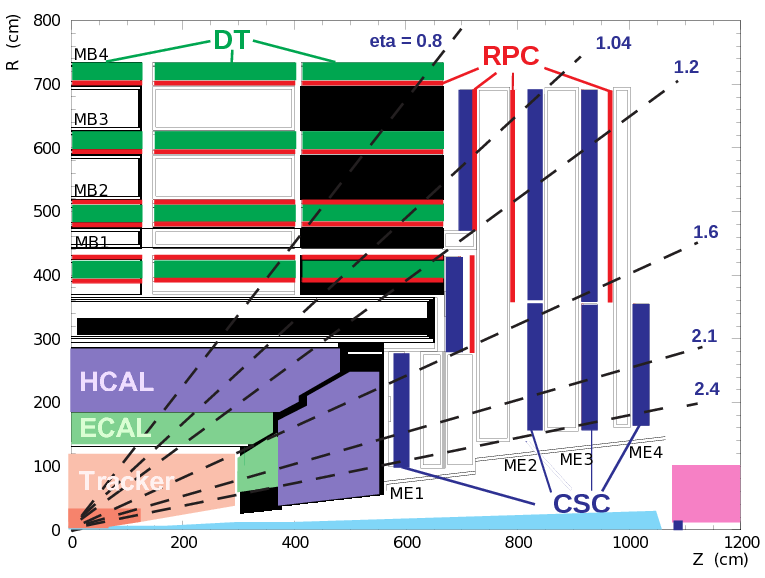
\includegraphics[width=0.85\textwidth]{figures/LHC/pictures_MuonSys-mod3.png}
	\caption{Longitudinal layout of one quadrant of the CMS detector. There are four DT stations named MB1-MB4 marked with green colour. Four CMS system in high pseudo-rapidity region named ME1-ME4 in blue colour. Also, there are several RPC stations in barrel region and part of endcap region marked with red colour.}
	\label{fig:muon-system-layout}
\end{figure}
Summary of CMS detector sub-system including its main characteristics and composition is given in Table~\ref{table:CMSMainChar}.
% subsection the_muon_system (end)
% subsection cms_sub_systems (end)
% % section cms_experiment (end)

\begin{table}
% \vspace{-5.2em}
\centering
\begin{tabular}[!htbp]{l l l}
\hline
{\bf Sub-system} & {\bf Composition} & {\bf Charateristics} \\
\hline
Tracker  & silicon strip and  & isolated track effiency $\epsilon > 95\%$ \\
	& pixel detector	& within jets $\epsilon \sim 90\%$ \\
	& 	& primary vertex resolution: 10-20 $\mu m$ \\
	& 	& $p_T$ resolution: $\Delta p_T/p_T = 1\%$ (0.1 TeV), 10\% (TeV)\\
	& 	& coverage $\eta<2.5$ \\
\hline
ECAL 	& 	$PbWO_4$ crystals 	& energy resolution:\\
		& 	& $\big(\frac{\sigma}{E}\big)^2 = \big(\frac{2.7\%}{\sqrt{E}}\big)^2 + \big(\frac{210}{E}\big)^2 + 0.55\% $  (barrel)\\
		& 	& $\big(\frac{\sigma}{E}\big)^2 = \big(\frac{5.7\%}{\sqrt{E}}\big)^2 + \big(\frac{245}{E}\big)^2 + 0.55\% $  (end-caps)\\
		& 	& coverage $\eta < 3$ \\
\hline
HCAL 	& 	Cu-Zn 	& energy resolution:\\
		& 	scintillators & $\big(\frac{\sigma}{E}\big)^2 = \big(\frac{68\%}{\sqrt{E}}\big)^2 + 4.5\%$ \\
		& 	& coverage $\eta < 3$ \\
\hline
Muon system & gaseous & efficiency $\epsilon \sim 98\%$ \\
			& detectors & $\Delta p_T/p_T =$8-15 \% (0.01 TeV)/20-40\% (TeV)\\
		& 	& coverage $\eta < 2.4$ \\
\hline
\end{tabular}
\caption{Main characteristics of the CMS sub-system~\cite{JeremieThesis}}
\label{table:CMSMainChar}
\end{table}


% %%%%%%%%%%%%%%%%%%%%%%%%%%%%%%%%%%%%%%%%%%%%%%%%%%%%%%%%%%%%%%%%%%
\subsection{CMS Trigger and Data Acquisition system} % (fold)
\label{sub:cms_trigger_and_data_acquisition_system}
The LHC produces 1 billion p-p collisions every second and thousands of particles produced during these collisions cross the CMS detector and reconstruction of these events generates several Terabytes of data. However, till now we neither have a switch with the required bandwidth that can transfer enormous data for further processing nor the disk space to store all of them. Even if we have one, then there are only a few fractions of data that are interesting for new physics or help to understand the existing one as most of the collisions is the low-energy glancing collision instead of head-on interaction. The maximum amount of data that can be stored every day is of the order of few Terabytes that decides the rate at which we can accept the events ($\sim$ 100 Hz).The concept of the trigger, method to select events of interest, was first introduced by ZEUS experiment~\cite{ZEUSCollaboration1993}, that handles data in real time, coupled with complex data acquisition system. While designing the trigger one has to keep in mind that trigger should efficiently accept the interesting physics while rejecting the non-interesting ones as whatever information lost at this level can not be recovered.

The CMS trigger system is divided into two steps, level 1 (L1) trigger which is a custom hardware process running synchronously with the LHC bunch crossing frequency of 40 MHz and the High-Level Trigger (HLT)~\cite{paper:JINST:CMSCollaboration}. The L1 trigger system analyses the events based on the information of calorimeter and muon system and  then selects the interesting events. However, this decision cannot take place within 25 ns, so a latency of 3.2 $\mu s$ was added. The maximum allowed frequency at the L1 stage is 100 kHz. Then the complete information is sent to HLT processing farm to reduced the event rate to $\sim$100 Hz. The remaining information is sent to Tier-0 centres to store and use it for offline analysis.



% section cms_trigger_and_data_acquisition_system (end)

% %%%%%%%%%%%%%%%%%%%%%%%%%%%%%%%%%%%%%%%%%%%%%%%%%%%%%%%%%%%%%%%%%%
\subsection{CMS Offline Computing} % (fold)
\label{sub:cms_offline_computing}
Once the data are selected by the trigger system, they are ready to be analysed offline. Before that, the raw data need to be processed, i.e., to convert data into understandable physics objects like electrons, muons, photons, jets, and so on. This step is known as object reconstruction which is the most CPU intensive task in the data processing chain of CMS. In this step one needs to reconstruct the primary vertices, charged particle tracks, identify electrons, photons, muons, reconstruct jets, apply b-tagging algorithm to reconstruct b-jets, run detector specific filtering and so on.
To perform all these steps CMS developed its software which is known as CMSSW. This software is based on Event Data Model (EDM) centred around the concept of the event. Here, an event is a C++ object container for all raw and reconstructed data related to a particular collision. Finally, these events are stored in ROOT files~\cite{Root1996}. The CMSSW event processing model consists of one executable called cmsRun, and many plug-in modules. These modules contain all the necessary codes for the event processing such as calibration and reconstruction algorithms~\cite{Bayatyan2005}.
To analyse data, we also need MC simulations which are carried out based on the predictions of SM and various new physics models. MC events are generated at parton level. Then showering and hadronization is applied, and finally, these events are put through the GEANT4~\cite{Agostinelli2003} based CMS detector simulation. The result is data similar to what one obtains from the actual detector. This MC data can then also be reconstructed as if it were  detector data.


% section cms_offline_computing (end)




% \begin{figure}[!htbp]
% 	\centering
% 	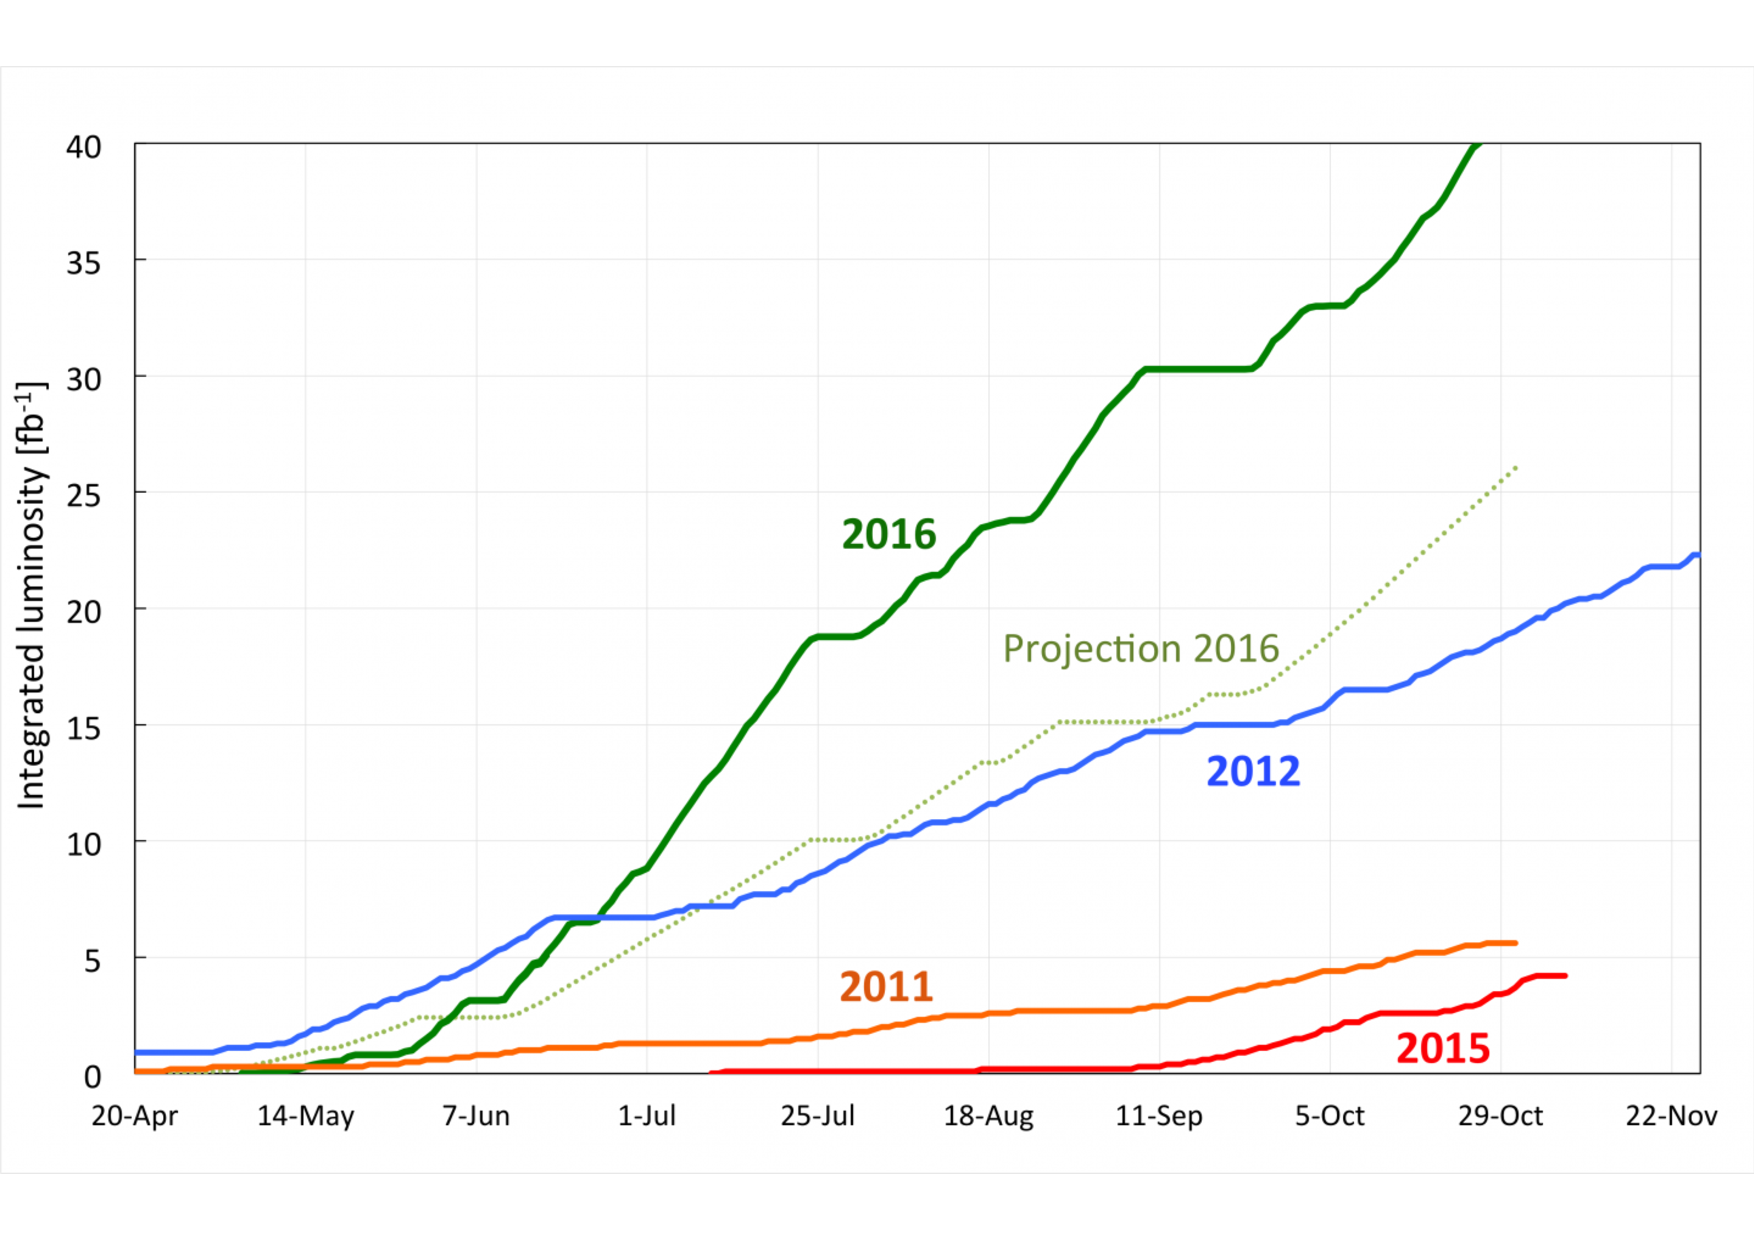
\includegraphics[width=0.95\textwidth]{figures/lumi-proj-2016-final-v2}
% 	\caption{The integrated luminosity of the LHC with proton-proton collisions in 2016 compared to previous years. Luminosity is a measure of a collider’s efficiency and is proportional to the number of collisions. The integrated luminosity achieved by the LHC in 2016 far surpassed expectations and is double that achieved at a lower energy in 2012. (Image : CERN)\todo[inline]{Update the caption.}}
% 	\label{fig:lumi-proj-2016-final-v2}
% \end{figure}





% Because of limited geometrical space in LHC ring the beam pipe was designed as a ``twin-aperture" magnets, where superconducing ring is housed in a common return yoke and cryostat.

% chapter the_lhc_and_cms_machine (end)


% \begin{figure}[!htbp]
% 	\centering
% 	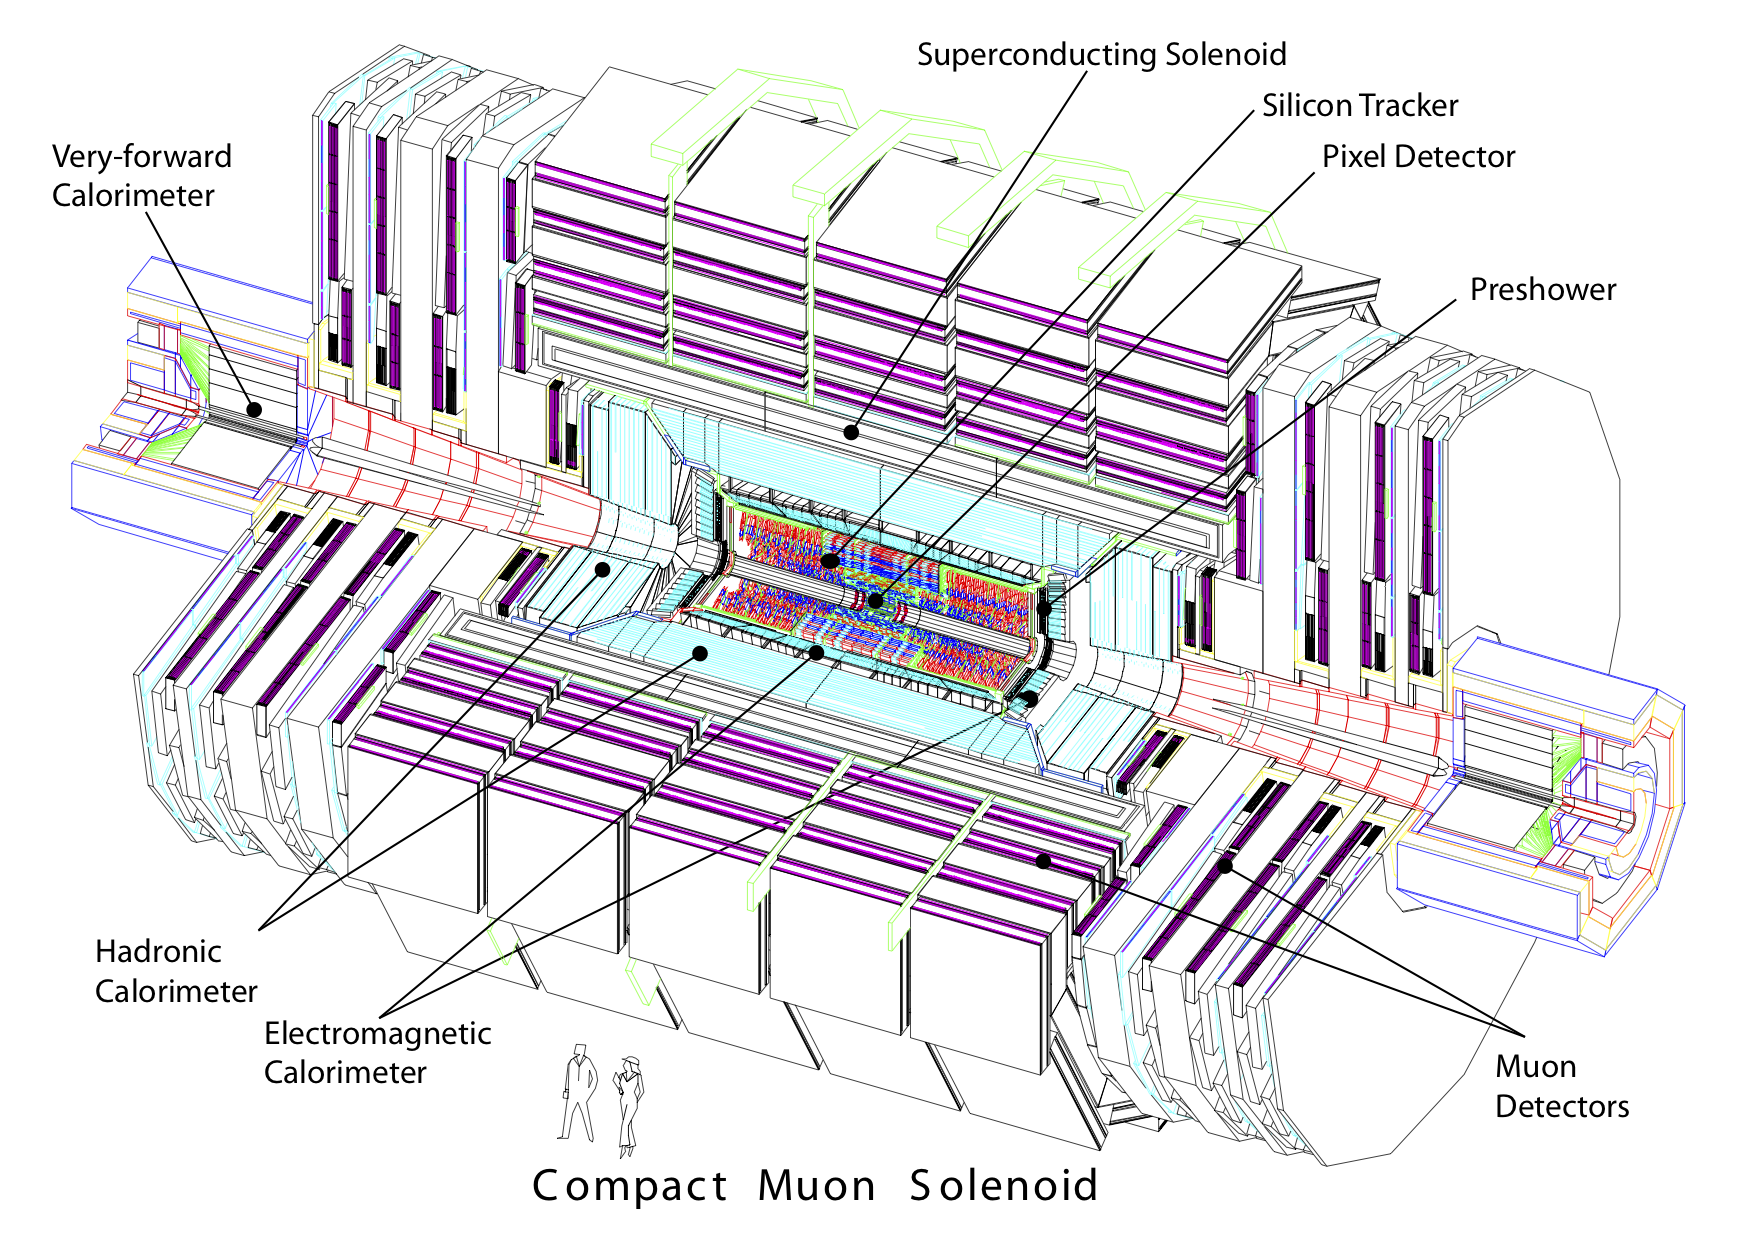
\includegraphics[width=0.95\textwidth]{figures/LHC/cms_complete_labelled.png}
% 	\caption{CMS detector drawing}
% 	\label{fig:CMS-detector-2}
% \end{figure}
